\section{Introduction}
\label{sec:intro}
Audio-driven talking head synthesis, which aims to generate realistic facial animations synchronized with audio, has become a key technology in digital humans and virtual reality~\cite{gafni2021dynamic, tan2024style2talker, tan2024say, chen2025echomimic, zhang2024tamm, zhang2025unleashing, yin2025trim, kumar2025charm3r, zhu2026fusionagent, zhu2026can, zhu2025quality, zielonka2023instant}. The advent of Neural Radiance Fields (NeRF)~\cite{mildenhall2021nerf} and 3D Gaussian Splatting (3DGS)~\cite{kerbl20233d} has significantly advanced 3D talking head synthesis~\cite{li2023efficient, ye2023geneface, li2024talkinggaussian, cho2024gaussiantalker, li2025instag, hou2024compose, liu2022blind}. But current 3D person-specific models~\cite{li2023efficient, li2024talkinggaussian, zhang2025fate, li2025rgbavatar} still rely on minute-level monocular videos and subject-wise optimization, which impedes rapid deployment and scalable personalization. 

A promising direction is the Pretrain-and-Adapt (PAA) paradigm that learns a universal audio-motion prior and adapts it to new identities using a few seconds of video. However, existing PAA-based pipelines~\cite{li2025instag, nie2025few} primarily focus on neutral speech scenarios with limited ability to capture emotion-driven facial motion, a central component of real-world human communication. Empirical evidence in Fig.~\ref{fig:mouth_open} further shows that emotional audio exhibits more complex motion dynamics than neutral audio, highlighting the need to model emotion-driven prosodic cues beyond phonemes. This raises a core question: \textit{Can few-shot 3D talking head synthesis move beyond neutral speech to support emotion-aware animation for expressive speech?}

\begin{figure}[t] 
\centering 
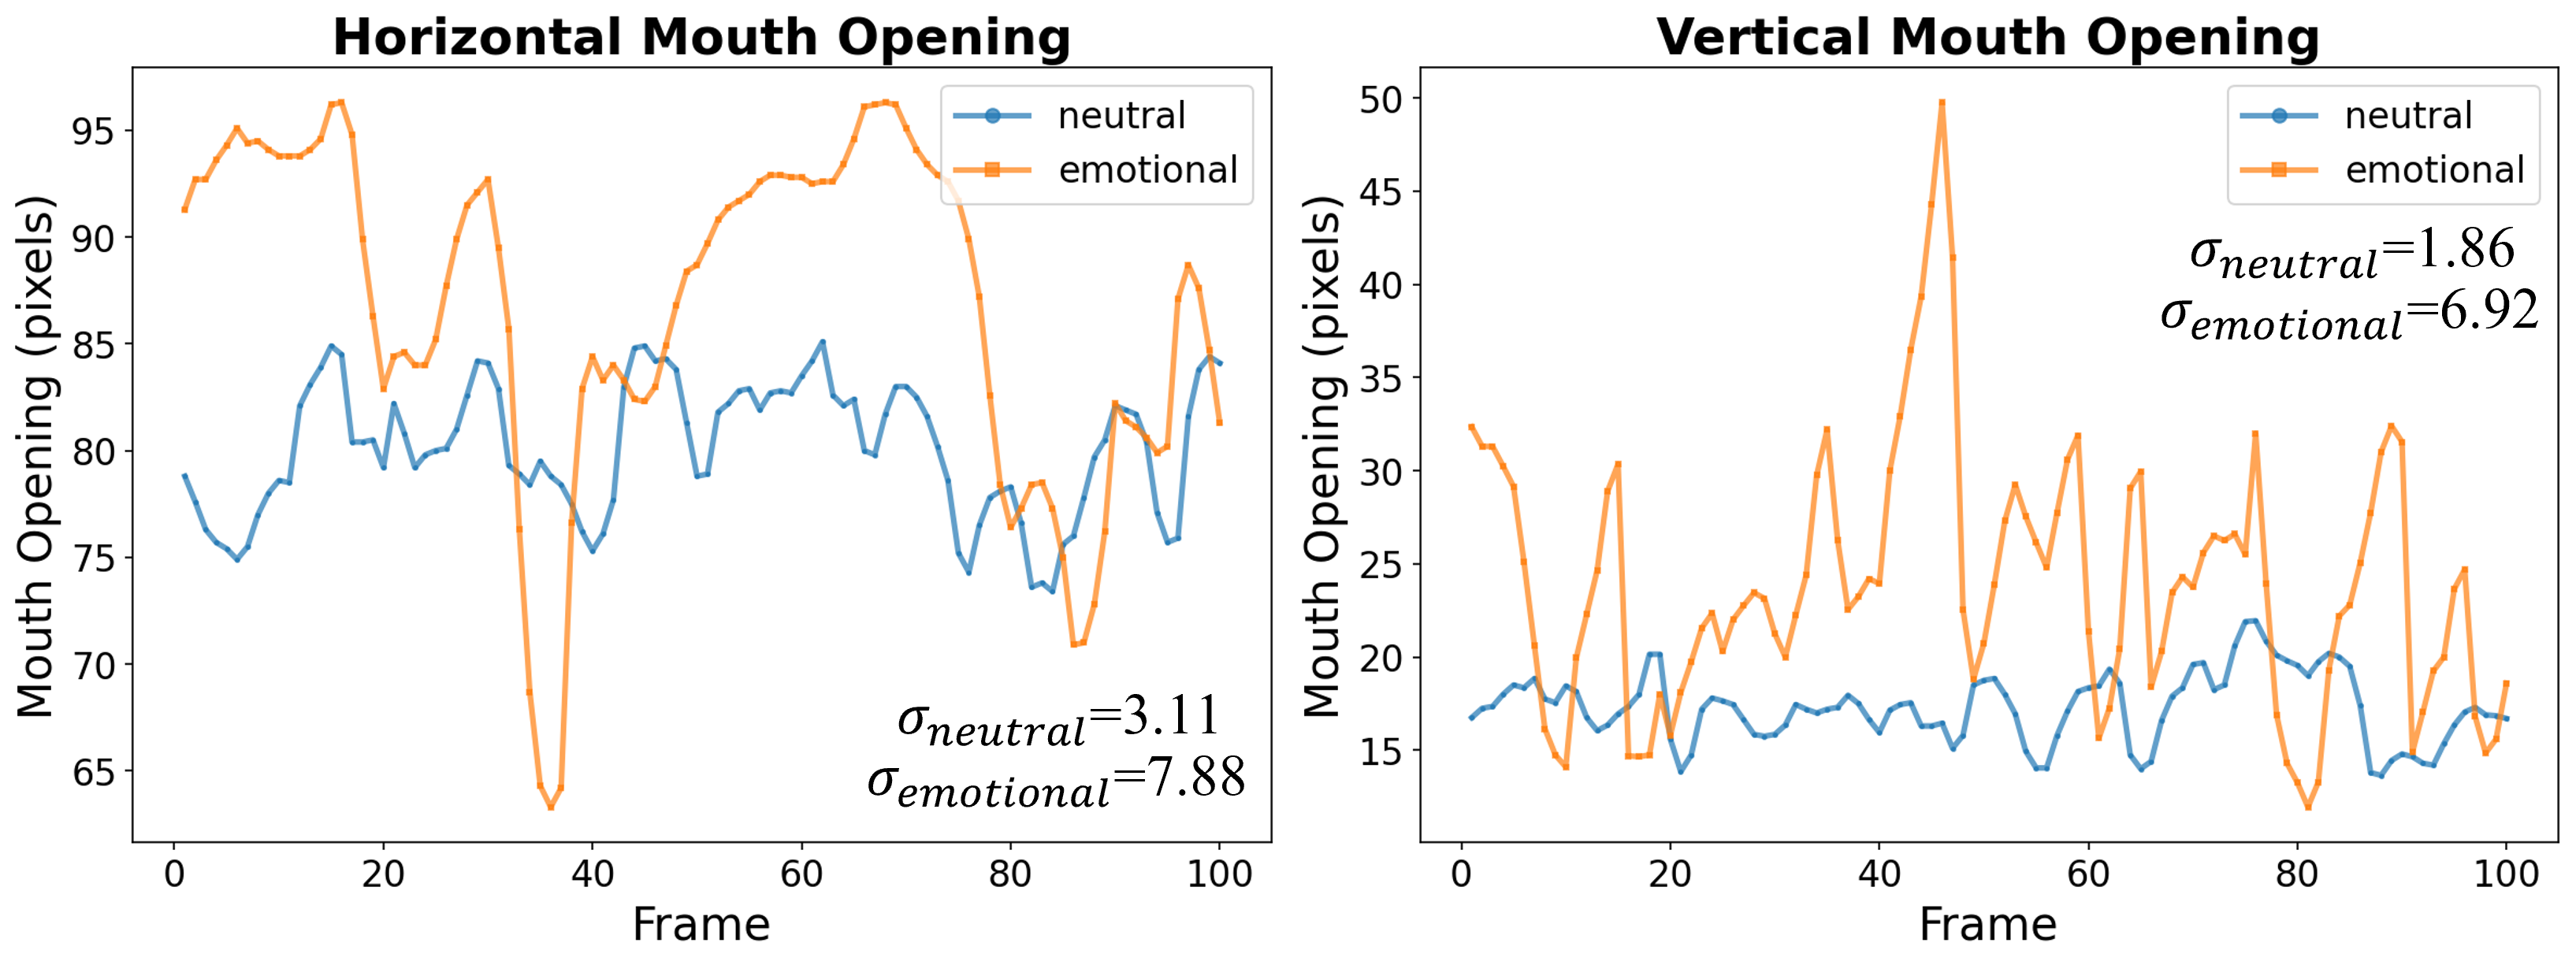
\includegraphics[width=\linewidth]{./Fig/mouth_open.png} 
\vspace{-15pt}
\caption{
\textbf{Neutral vs emotional articulation complexity.} 
We compare horizontal and vertical mouth opening trajectories measured from lip landmarks. 
Emotional audio shows stronger temporal fluctuation and larger standard deviations (\(\sigma_{\text{emotional}}=7.88, 6.92\)) than neutral audio (\(\sigma_{\text{neutral}}=3.11, 1.86\)), 
revealing more complex articulation patterns.
}
\vspace{-10pt}
\label{fig:mouth_open} 
\end{figure}

To answer this question, we propose Emotion-Aware Talking Head Synthesis on Gaussian Splatting \textbf{(EmoTaG)}, a framework for emotion-aware and structurally consistent 3D talking head synthesis with few-shot personalization, as shown in Fig.~\ref{teaser}.
Specifically, we adopt FLAME~\cite{li2017learning} as an explicit geometric prior and predict its expression and jaw parameters. These predicted parameters deform the FLAME mesh and drive rigged 3D Gaussians through a FLAME-Gaussian formulation~\cite{qian2024gaussianavatars} for stable facial motion. Intra-oral regions are further refined using mouth Gaussians selected by lip landmarks, which capture fine-grained articulations such as teeth and tongue movements.
Building on this, we propose a Gated Residual Motion Network (GRMN) composed of an Identity-Conditioned Encoder and an Expert Motion Decoder. The encoder integrates prosody-aware audio features and upper-face Action Unit cues to capture emotion-related dynamics, while incorporating an identity embedding through AdaIN-based modulation~\cite{huang2017arbitrary, karras2019style} for personalized feature adaptation. The decoder contains three cooperative branches: a base branch that captures phonetic audio-motion mapping, a residual branch that models emotion-related and identity-specific variations, and a gate branch that adaptively combines the base and residual outputs to produce stable and expressive facial motion. To enhance emotional sensitivity, we further introduce Semantic Emotion Guidance, which distills the emotion distribution and emotion intensity score from a pretrained emotion recognizer named DeepFace~\cite{serengil2024lightface} into the GRMN’s residual and gate branches, enabling emotion-aware motion learning without manual annotations.

Our main contributions are summarized as follows:
\begin{itemize}
\item We propose \textbf{EmoTaG}, a framework for emotion-aware and stable few-shot 3D talking head synthesis that adapts to a new identity using only 5 seconds of video.
\item We design a Gated Residual Motion Network that separates phonetic articulation from emotion-related motion and adaptively fuses them through a gating mechanism. We further introduce Semantic Emotion Guidance, which distills semantic emotion knowledge from a pretrained emotion recognizer to enable emotion-aware motion learning without manual annotations.
\item Extensive experiments show that EmoTaG achieves state-of-the-art performance in emotional expressiveness, lip synchronization, visual realism, and motion stability across diverse evaluation scenarios.
\end{itemize}

\begin{figure*}[ht]
    \centering
    
\includegraphics[width=1\textwidth]{./Fig/pipeline.png}
    \vspace{-15pt}
    \caption{
\textbf{Overview of EmoTaG.} 
For pretraining, our Gated Residual Motion Network learns a universal motion prior from a multi-identity corpus. This network comprises an Identity-Conditioned Encoder for integrating audio, expression, and identity through AdaIN-based modulation, followed by an Expert Motion Decoder that leverages emotion-distilled supervision to train three cooperative branches (Base, Residual, Gate). During adaptation, the Gated Residual Motion Network is efficiently adapted to a new identity from 5-second video via only tuning the AdaIN modulation parameters. At inference, the adapted model produces expressive, high-fidelity 3D facial animation driven by new audio with head pose and upper-face cues.
}
    \vspace{-10pt}
    \label{pipeline}
\end{figure*}

